\documentclass[12pt]{article}
\usepackage[utf8]{inputenc}
\usepackage{mathpazo}
\usepackage{subfig}
\usepackage[a4paper,top=3cm,bottom=3cm,left=2.5cm,right=2.5cm,marginparwidth=3cm]{geometry}
\pagestyle{myheadings}	\usepackage{tabularx}

% Paquetes
\usepackage{mathtools, amsmath, setspace, amsfonts, enumitem, listings}
\usepackage{cancel, amssymb, xfrac, enumitem, setspace, tcolorbox}
\usepackage{pdfpages, soul, graphicx, multicol, float}
\tcbuselibrary{theorems}

% Bibliography
\usepackage[spanish]{babel}
\usepackage[natbibapa]{apacite}
\bibliographystyle{apacite}

\usepackage[natbibapa]{apacite}
\bibliographystyle{apacite}

% Hipervinculos
\definecolor{udesa}{HTML}{00529B}
\usepackage[colorlinks=true, allcolors=udesa]{hyperref}
\usepackage{listings}
\usepackage[colorinlistoftodos]{todonotes}
\usepackage{parskip}

\DeclareMathOperator*{\plim}{plim}
\setlength{\parskip}{1em}

% Commands
\providecommand{\abs}[1]{\lvert#1\rvert}
\providecommand{\abs}[1]{\lvert#1\rvert}
\newcommand{\HRule}{\rule{\linewidth}{0.3mm}} 

\hypersetup{breaklinks=true,
            pdfauthor={Riquelme y Pacheco},
            pdftitle={Problem Set 2},
            colorlinks=true,
            citecolor=udesa,
            urlcolor=udesa,
            linkcolor=udesa,
            pdfborder={0 0 0}}


\markboth{4444}{Herramientas computacionales para la investigaci\'on - MAE UdeSA 2022}

\title{ %\includegraphics[scale=0.5]{Logos/Udesa_Azul.jpg}\\
%\vspace{0.5cm}
Herramientas computacionales para la investigaci\'on \\
\vspace{0.3cm}
\textbf{Tarea: QGIS }}
\author{Tom\'as Pacheco y Abigail Riquelme}
\date{Fecha de entrega 10/07/2022}

\begin{document}
\maketitle
\onehalfspace





\subsection*{Ejercicio 1}

Para comenzar a hacer los mapas tuvimos que cargar las dos bases de datos a QGIS. A continuación, nuestra próxima tarea era mergearlas por el id de área. En la base con los \textit{boundaries}, nos encontramos que la variable que indica el id estaba en formato string, por lo que tuvimos que generar una nueva variable que contuviese la misma información pero con formato numérico (\textit{integer}). Pars esto utilizamos la función \texttt{to\_int()}. Luego, juntamos ambas bases de datos y la exportamos con el nombre \texttt{data\_merge}.

En el primer gráfico (Figura \ref{precioairbnb}) presentamos el precio por persona de Airbnb (USD) en las diferentes comunidades de Chicago. Nos pareció interesante observar la distribución de los precios a lo largo del territorio nombrado con el objetivo de reconocer zonas en las que los precios son más altos o más bajos. Al momento de decidir la división de las categorías de los precios nos enfrentamos a un \textit{trade-off} entre presentar los datos de una manera más desagregada (con más categorías) y presentar el mapa de una forma más parsimoniosa. Teniendo en cuenta esto decidimos observar el mínimo y el máximo de los precios disponibles en nuestra base de datos y la distribución de esta variable (Figura \ref{histprecios}, más adelante comentaremos este gráfico en particular). A partir de esta información consideramos que dividir los precios de a 30 dólares era una buena manera de considerar varias categorías (seis) pero sin hacer demasiado compleja la lectura del gráfico. 

Al observar la Figura (\ref{precioairbnb}) notamos que la zona noreste de Chicago tiene los precio más elevados. En cambio en el sur es posible notar precios de las categorías más bajas. 


También consideramos interesante observar la cantidad de crímenes cada 100.000 habitantes en las comunidades de Chicago dado que este podría ser un indicador de la seguridad de cada comunidad. La base de datos contaba solo con la cantidad de crímenes, en donde se incluían los crímenes por agresión, robo, apuestas, homicidio, secuestro, robo, acecho, homicidio y hurto, entre otros. Por lo tanto, lo que hicimos fue crear la variable nombrada anteriormente. Consideramos que esto es necesario dado que es natural pensar que en aquellas comunidades en donde hay una población mayor observemos más crímenes. Luego de construir la variable realizamos el segundo mapa (Figura \ref{crimeneschicago}). 

Con respecto a la división en categorías decidimos dividir a nuestra variable en seis categorías mediante un conteo igual (quantil) de esta forma logramos diferenciar entre comunidades con mayor cantidad de crímenes por 100.000 habitantes y comunidades con menor cantidad de crímenes pero sin hacer el gráfico muy complejo en términos de la desagregación de categorías. 


Cuando hacemos un mapa por cuantiles se intenta tener la misma cantidad de observaciones en cada clase. En este caso lo que se hace es tomar la cantidad de comunidades (77). Luego se divide este número por la cantidad de clases. Por último, el mapa por cuantiles tiene ese porcentaje de observaciones en cada categoría. Realizamos un histograma y observamos que parece ser razonable la división propuesta obtenida mediante este método ya que se diferencian claramente las categorías. 


Al observar la Figura (\ref{crimeneschicago}) notamos que en el sur y centro de Chicago las comunidades tienen mayor cantidad de crímenes cada 100.000 habitantes que las comunidades del norte.

Por último, consideramos relevante observar la calificación promedio al \textit{host} de Airbnb para cada una de las comunidades de Chicago dado que podría ser un indicador de la calidad de las viviendas. Con este objetivo realizamos el tercer mapa (Figura \ref{califairbnb}). Para esto dividimos en 5 grupos de calificaciones, cada una con el mismo intervalo. Es interesante observar que no hay casos en los que la calificación promedio sea menor a 80. La Figura (\ref{crimeneschicago}) muestra que las comunidades del sur tienen menones calificaciones al \textit{host} de Airbnb que las comunidades del norte a excepción de la comunidad Ohare que está dentro del grupo con menor calificación (80 a 84). 


Posteriormente realizamos gráficos con los datos disponibles. En primer lugar, consideramos interesante realizar un histograma de los precios por persona de Airbnb en Chicago (Figura \ref{histprecios}). Se observa una mayor presencia de observaciones en entre los precios 60 y 80, es decir, que hay una mayor cantidad de comunidades con estos precios. Además, en la cola derecha de la distribución hay una menor cantidad de observaciones (80 a 180) que en la cola izquierda (0 a 60).


En segundo lugar, consideramos relevante ver si existe algún tipo de relación entre los datos de la tasa de desempleo y crímenes de las comunidades de Chicago. Con este objetivo realizamos un histograma 2D entre la tasa de desempleo y crímenes (Figura \ref{hist2dcrimunep}). En particular observamos que hay 10 estamos que tienen menos de 10\% de desempleo y entre 0 y 20.000 crímenes cada 100.000 personas. Además, hay cerca de 18 comunidades que tienen una tasa de desempleo que se encuentra entre el 10 y 20\% y a la vez entre 10.000 y 20.000 crímenes cada 100.000 personas. Para el resto de los casos la cantidad de comunidades oscila entre 0 y 8. 





Por último, nos interesó ver si se podía identificar algún tipo de relación entre el precio per cápita por alojamiento y los crímenes cada 100.000 habitantes en las comunidades de Chicago. Esperaríamos encontrar que a mayor cantidad de crímenes es menor el precio per cápita del alojamiento. Observamos una leve relación negativa entre los datos, aunque no es del todo evidente (Figura \ref{scatterpreciocrimen}). Es importante aclarar que se observa una gran dispersión de los datos. 









\begin{figure}
    \centering
    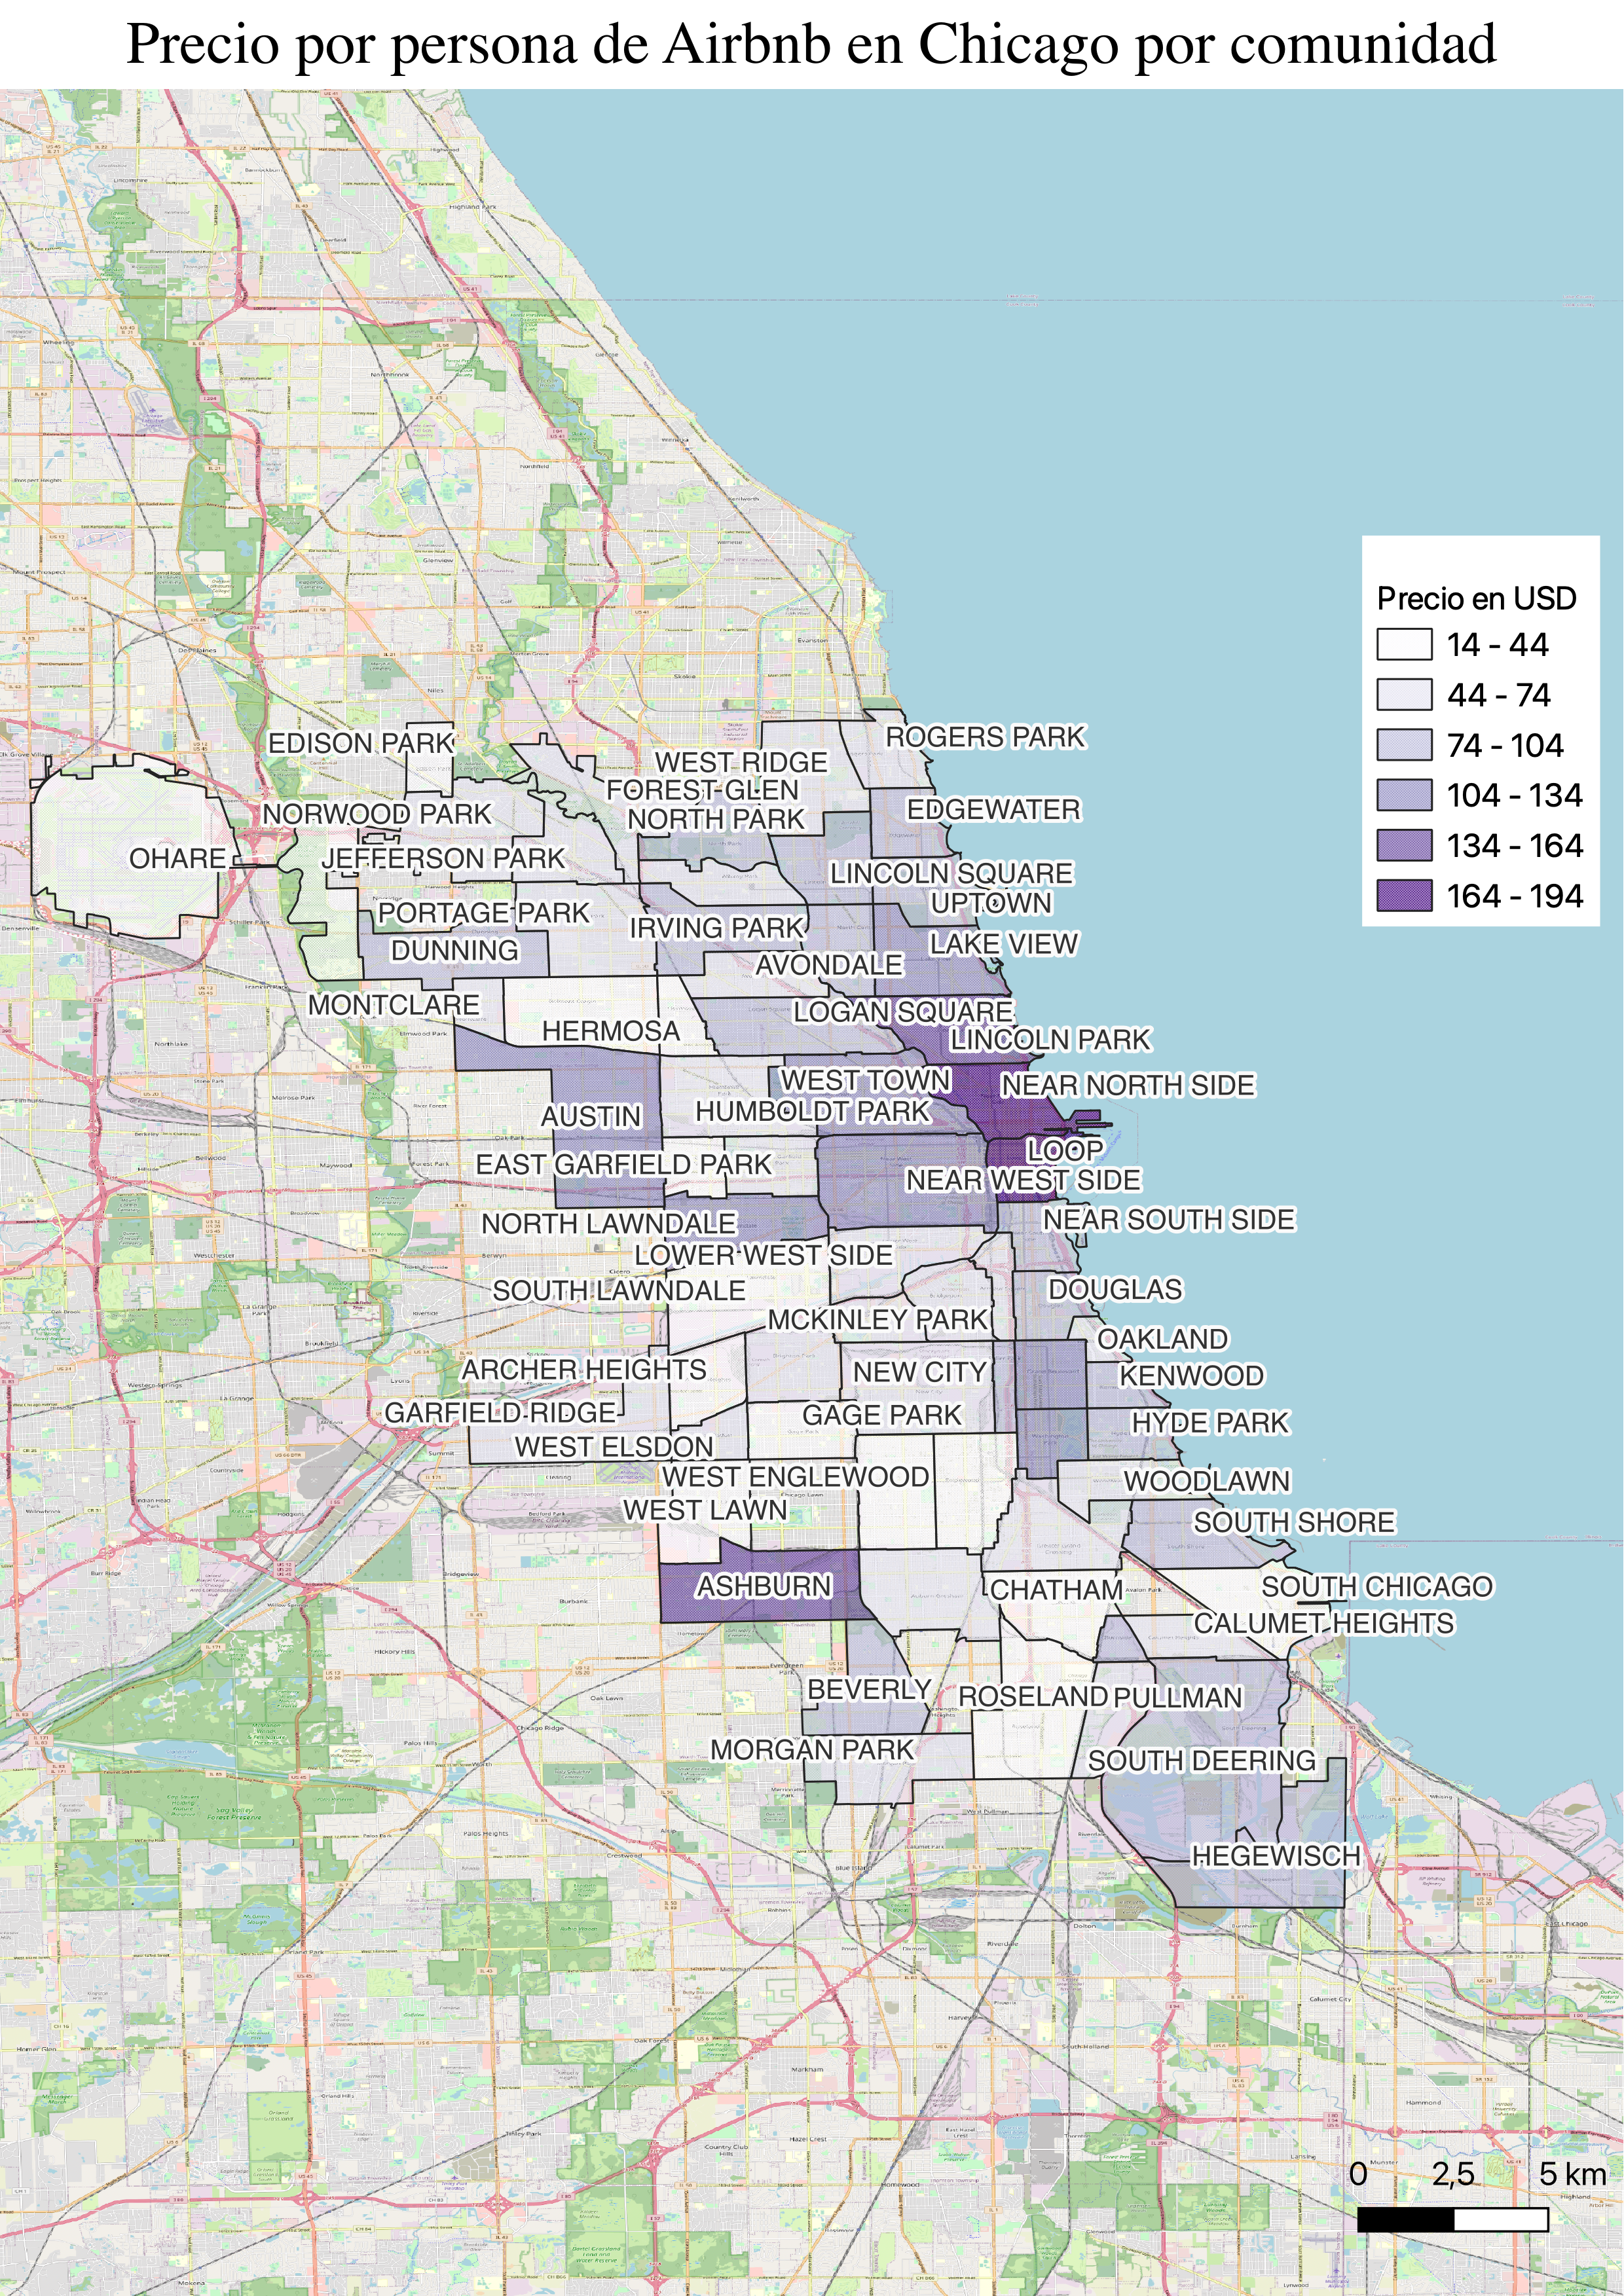
\includegraphics[scale = 0.8]{mapas/Chicago_Airbnb_Precio.png}    \caption{Precio per c\'apita del alojamiento}
    \label{precioairbnb}
\end{figure}

\begin{figure}
    \centering
    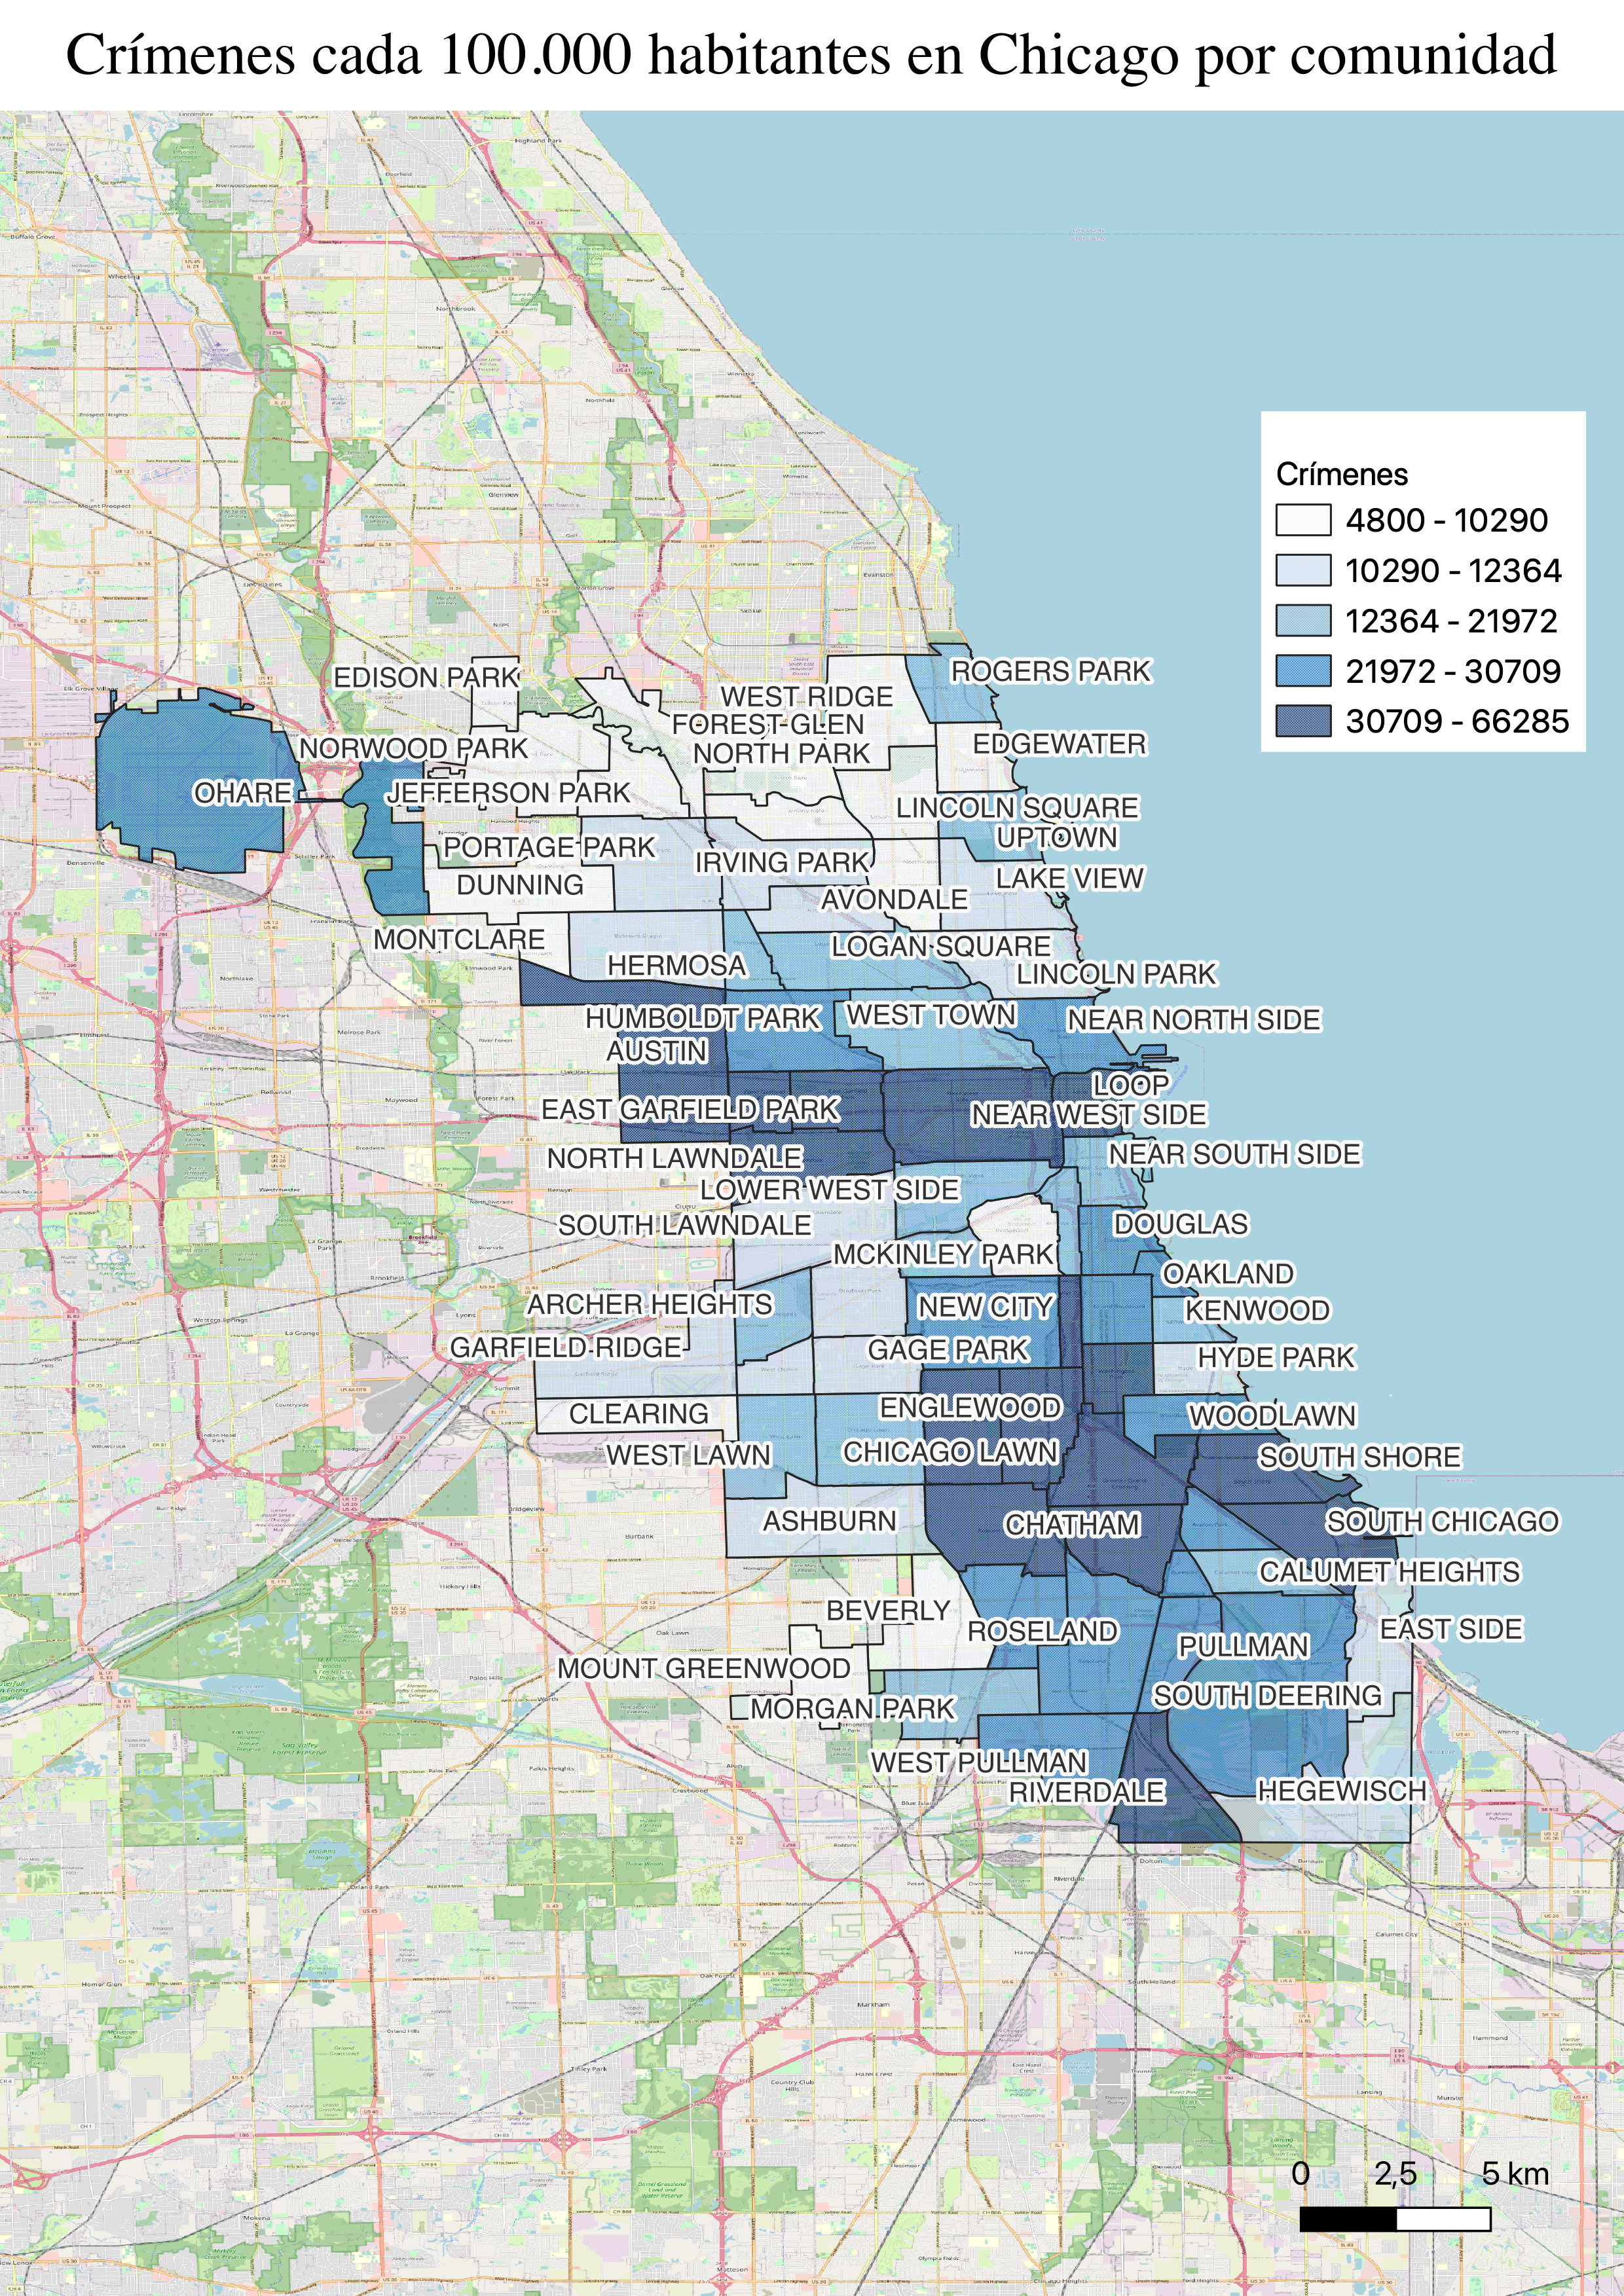
\includegraphics[scale = 0.8]{mapas/Chicago_crimenes.png}    \caption{Cr\'imenes cada 100.000 habitantes}
    \label{crimeneschicago}
\end{figure}

\begin{figure}
    \centering
    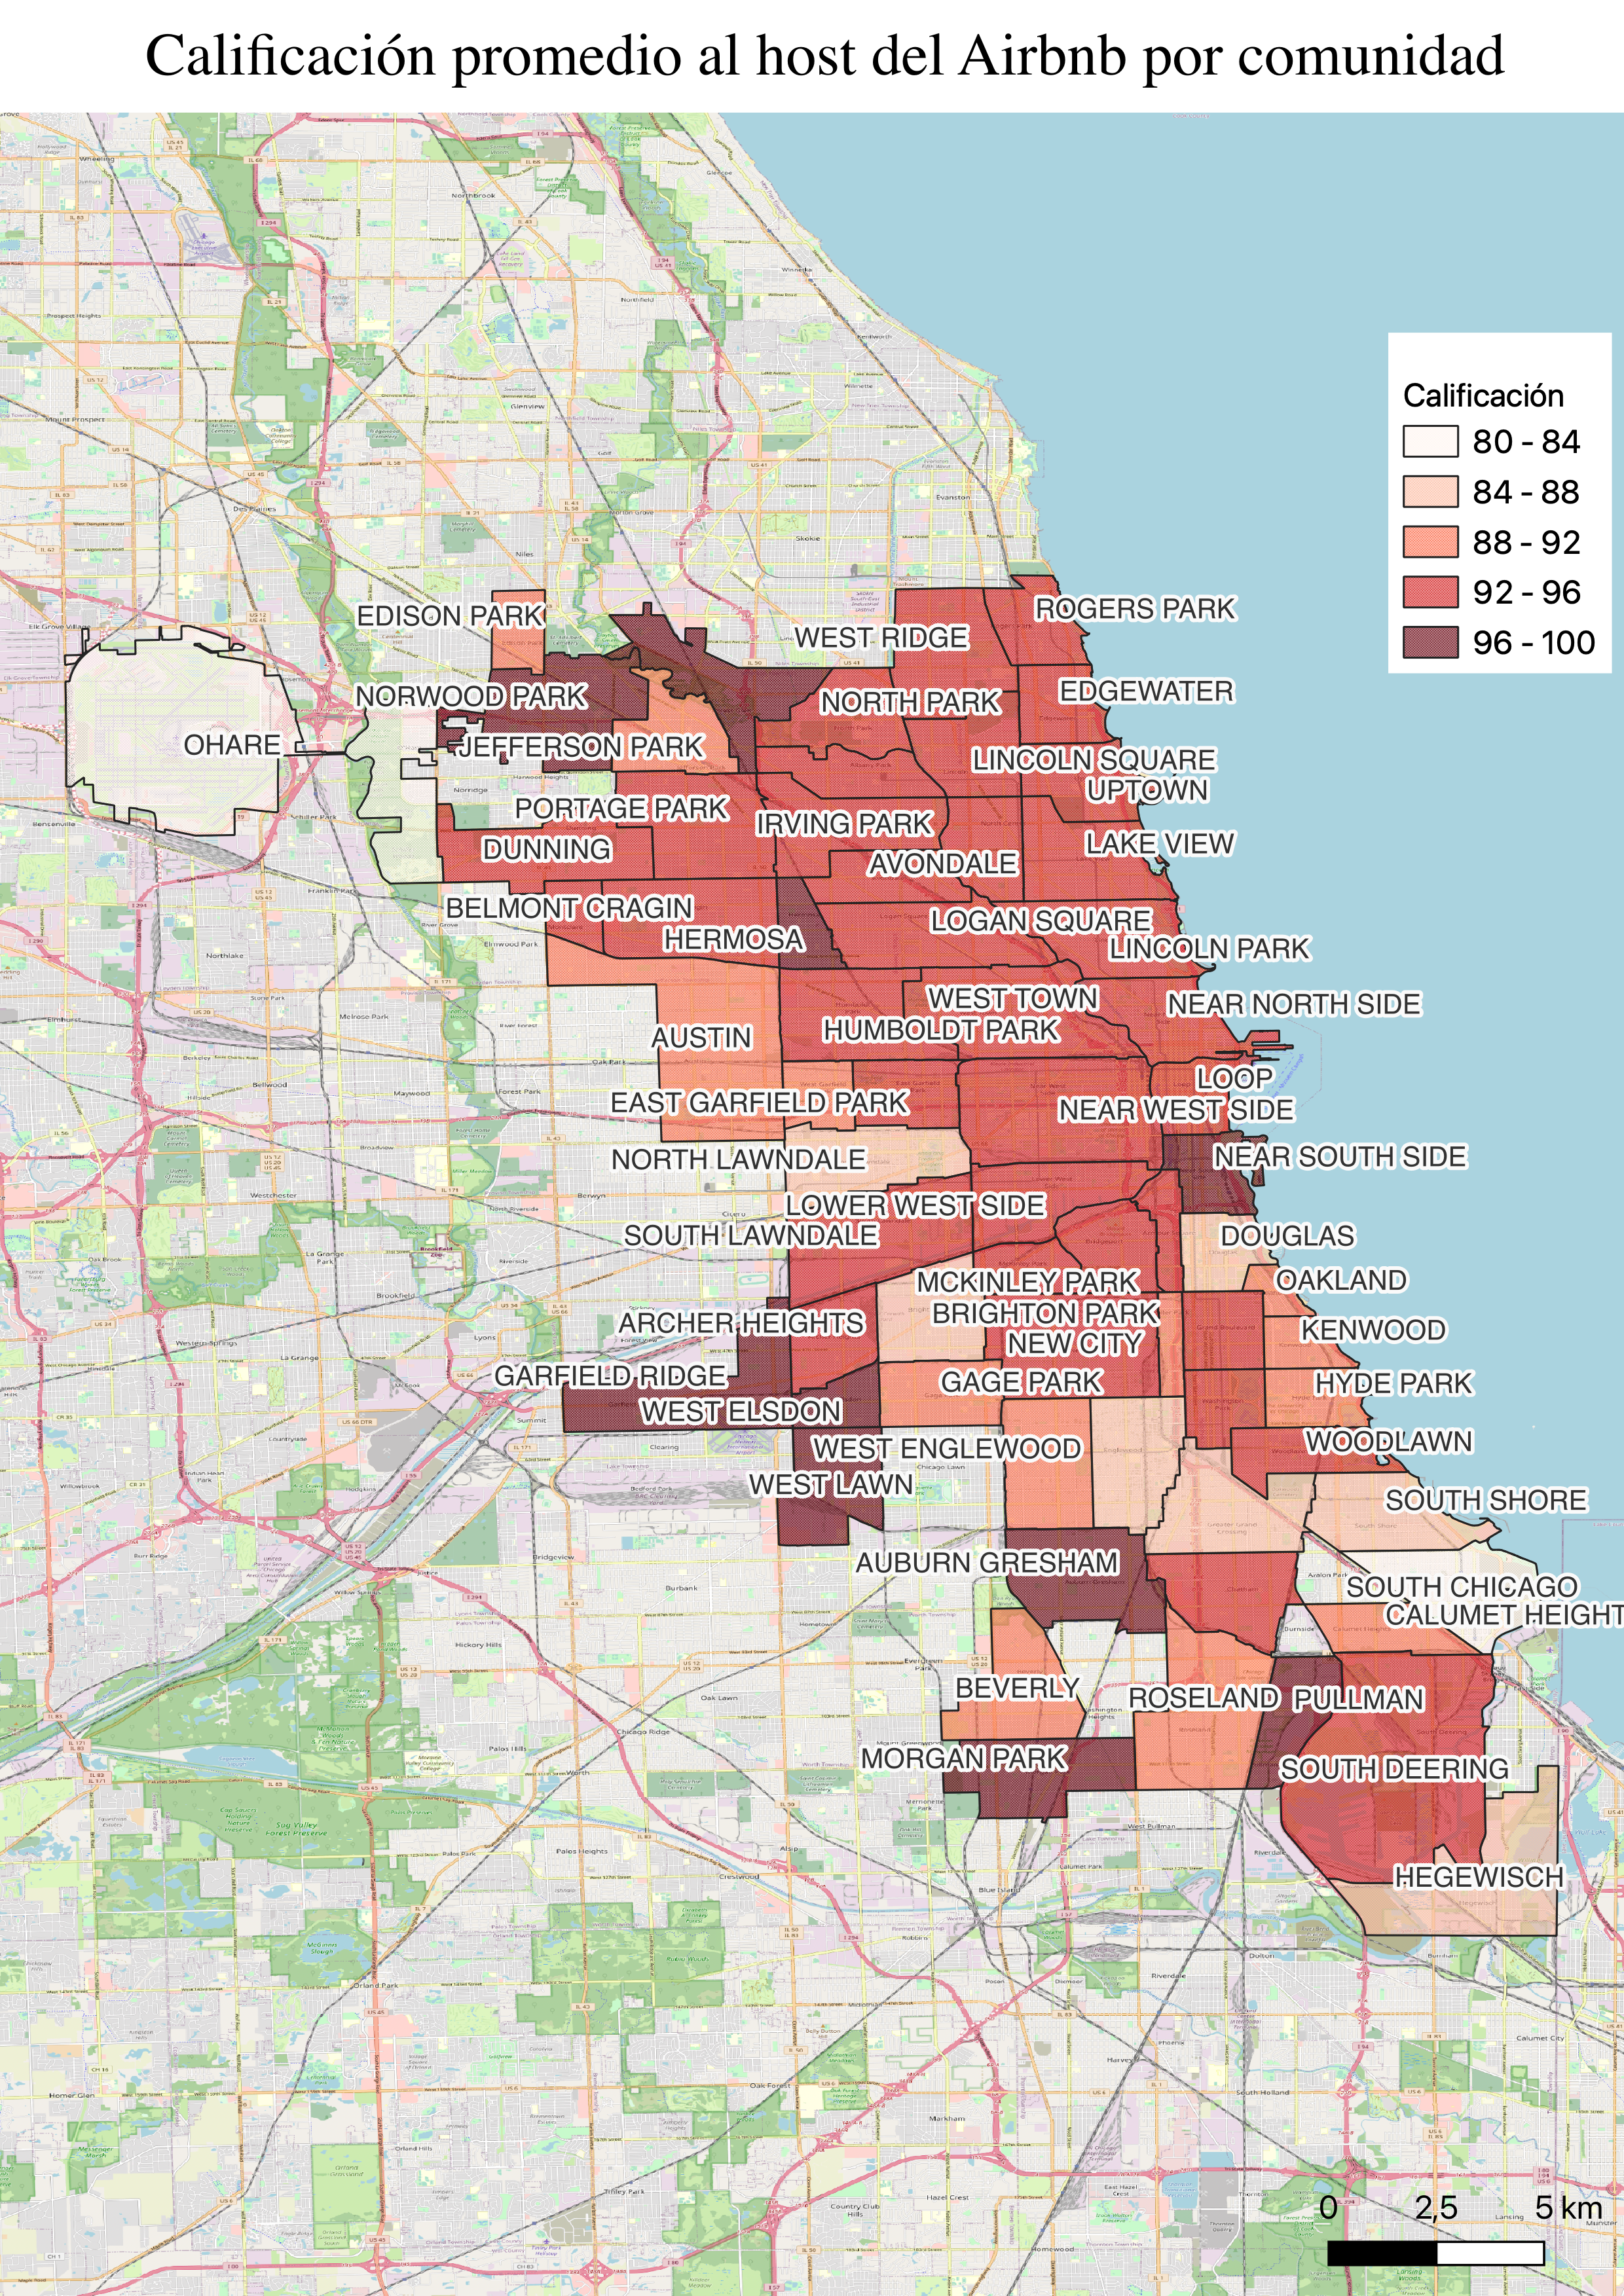
\includegraphics[scale = 0.8]{mapas/Chicago_Airbnb_Califprom.png}   
    \caption{Rating promedio al \textit{host} del Airbnb en Chicago}
    \label{califairbnb}
\end{figure}



\begin{figure}
    \centering
    \includegraphics[width = \textwidth]{mapas/Chicago_Hist_Precio.png}   
    \caption{Histograma de precios por persona}
    \label{histprecios}
\end{figure}

\begin{figure}
    \centering
    \includegraphics[width = \textwidth]{mapas/Chicago_Corr_CrimenesUnemp.png}   
    \caption{Histograma 2D de crímenes y desempleo}
    \label{hist2dcrimunep}
\end{figure}

\begin{figure}
    \centering
    \includegraphics[width = \textwidth]{mapas/Chicago_Scatter_PrecioCrimenes.png}   
    \caption{Diagrama de dispersi\'on entre cr\'imenes y precios}
    \label{scatterpreciocrimen}
\end{figure}









\subsection*{Ejercicio 2}

En este punto trabajamos con una base de datos de Argentina para graficar estadísticas de cada uno de los partidos de la Provincia de Buenos Aires. Comenzamos descargando los datos cartográficos del sitio web del \href{https://www.indec.gob.ar/indec/web/Institucional-Indec-Codgeo}{INDEC}. Luego, tambi\'en de la p\'agina web del INDEC, m\'as espec\'ificamente de la base de datos \href{https://redatam.indec.gob.ar/argbin/RpWebEngine.exe/PortalAction?&MODE=MAIN&BASE=CPV2010A&MAIN=WebServerMain.inl&_ga=2.11555124.1497521223.1592814315-345592181.1592814315}{REDATAM}, descargamos dos indicadores. El primero de ellos es la condici\'on de actividad para cada uno de los departamentos de la provincia. El segundo, es uno que indica si los hogares tienen al menos un indicador de necesidades b\'asicas insatisfechas. A estas bases de datos tuvimos que limpiarlas utilizando el \textit{do file} provisto. Luego, las importamos al QGIS y juntamos todo para poder graficar los dos mapas que explicaremos a continuaci\'on.
    

En el primer mapa (Figura \ref{bsasnbi}) mostramos el porcentaje de hogares con algún indicador de necesidades básicas insatisfechas por partido de la Provincia de Buenos Aires. Para dividir en categorías utilizamos la clasificación de cortes naturales Jenks. En este caso las diferentes categorías se basan en las agrupaciones naturales de los datos. Lo que se busca es que tener dentro de cada clase los valores similares que mejor se agrupan y que a la vez se maximicen las diferencias entre categorías. \\


La clasificación nombrada anteriormente está basada en el algoritmo de rupturas naturales de Jenks. Lo que primero que hace este algorítmo es trabajar con la variable o atributo a clasificar ($y$) y la cantidad de categorías que son elegidas por el investigador ($k$). Luego, se genera un conjunto de $k-1$ valores aleatorios o uniformes en el rango $[\min \{y\}, \max\{y\}]$. Estos se utilizan como los límites de las categorías iniciales. Posteriormente se calculan los valores medio para cada categoría inicial y se calcula la suma de las desviaciones al cuadrado de las observaciones de la categoría con respecto a los valores medios correspondientes. Se registra la suma total de las desviaciones al cuadrado. Luego, se asigna de manera sistemática los valores individuales a las categorías ajustando los límites de las categorías para ver si es posible reducir la suma total de las desviaciones al cuadrado. Este es un proceso iterativo que finaliza cuando la varianza dentro de cada categoría es lo más pequeña posible y la varianza entre clases es lo mayor posible \citep{de2007geospatial}. 


Al utilizar la clasificación de cortes naturales de Jenks para seis categorías obtenemos los rangos específicados en la Figura (\ref{bsasnbi}). Observamos que en el centro de la Provincia de Buenos Aires los valores son relativamente bajos, es decir, el porcentaje de hogares con alg\'un indicador de necesidades b\'asicas instafisfechas oscila entre el 1,1 y 4,7\%. En cambio, en los partidos más alejados el porcentaje de hogares con algún indicador de necesidades básicas insatisfechas aumenta. Por ejemplo, al sur de la provincia, se puede ver que los partidos de Villarino y Patagones tienen un elevado porcentaje de hogares sin alguna necesidad b\'asica cubierta. El porcentaje est\'a entre el 13,6 y 18,4\% para Villarino y 4,7 y 7\% para Patagones. Otro ejemplo es lo que sucede al este de la provincia, en el que algunos partidos de la costa, como Tordillo, La Costa, Pinamar y Villa Gesell tienen una proporci\'on mayor comparada a la de los partidos vecinos. Por \'ultimo, podemos decir que algo similar sucede en el conurbano, en donde los partidos que rodean a la Ciudad de Buenos Aires, tienen valores mayores para el indicador en cuesti\'on.

\begin{figure}
    \centering
    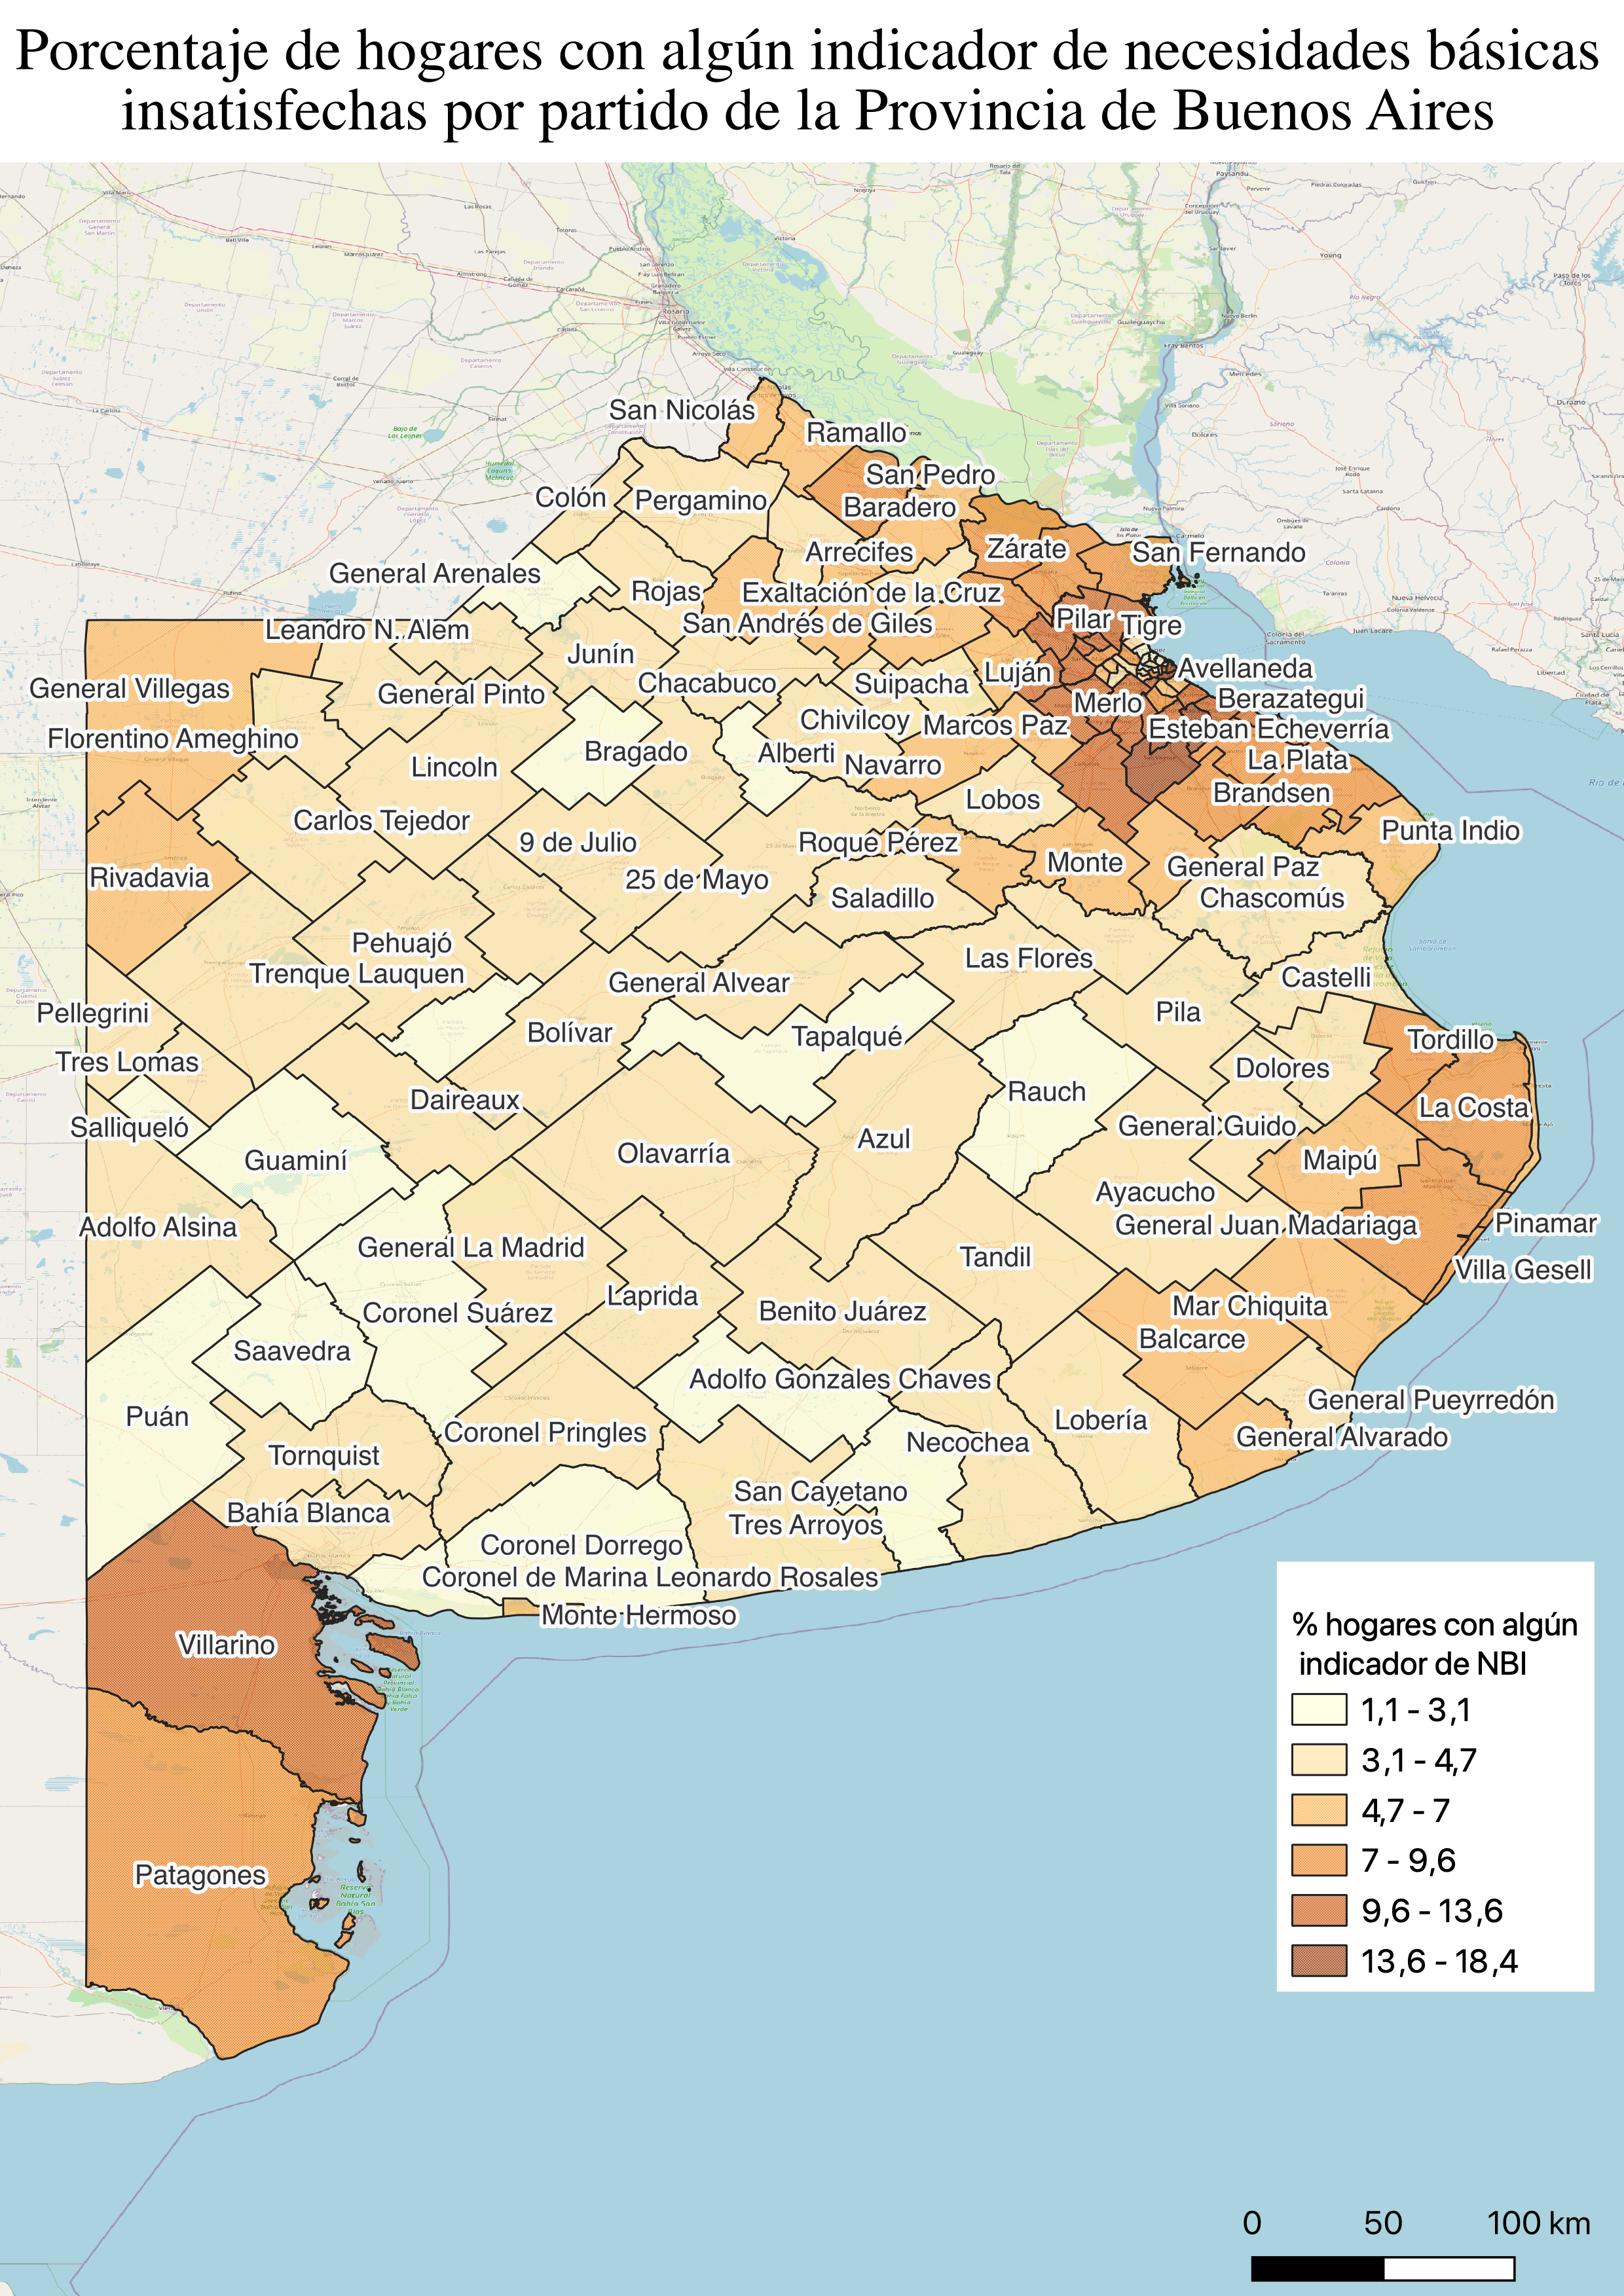
\includegraphics[scale = 0.8]{mapas/Pcia_BsAs_NBI.png}   
    \caption{Porcentaje de hogares con algún indicador de NBI}
    \label{bsasnbi}
\end{figure}

En el gr\'afico que realizamos anteriormente pod\'iamos distinguir, a trav\'es de la escala de colores, los distintos valores que puede tomar el indicador para cada categor\'ia. Sin embargo, una limitaci\'on que tienen estos tipos de mapas (o tal vez la escala elegida), es que no se pueden observar las diferencias dentro de cada una de las categor\'ias. Es por esto que para mostrar la tasa de desempleo  por partido de la Provincia de Buenos Aires, decidimos hacer un gr\'afico 3D (Figura \ref{bsasundemp}). Este tipo de gr\'afico viene a solucionar el problema recientemente mencionado: se pueden ver las diferencias dentro de cada una de las categor\'ias.

Para nuestro mapa, decidimos dividir en seis categorías de igual magnitud para poder distinguir mediante colores entre estos grupos. De esta forma en el gráfico podemos observar mediante la altura la diferencia de los valores de la tasa de desempleo por partido entre los partidos que están en una misma categoría. En la Figura (\ref{bsasundemp}) observamos que los partidos del centro y del oeste de la provincia son los que tiene una menor tasa de desempleo en comparación a los partidos que se encuentran en los bordes de la provincia. Este patrón es similar al encontrado en la Figura (\ref{bsasnbi}). Por ejemplo, Villarino es el partido que mayor tasa de desempleo tiene. Lo mismo sucede con algunos partidos de la costa este y de la zona del conurbano. Es posible pensar que esto tiene sentido debido a que tener alguna necesidad básica insatisfecha podría ser más probable si una persona está desempleada. 

\begin{figure}
    \centering
    \includegraphics[width = \textwidth]{mapas/Pcia_BsAs_Desempleo.png}   
    \caption{Tasa de desempleo por partido}
    \label{bsasundemp}
\end{figure}






%\newpage
\bibliography{ref}
%\nocite{*}




\end{document}




